\documentclass[a4paper,12pt]{article}
\usepackage{../../mypackages}
\usepackage{../../macros}

% \definecolor{SectionColor}{HTML}{1A73E8}      % Blue
% \definecolor{SubsectionColor}{HTML}{EA4335}   % Red

\DeclareUnicodeCharacter{202F}{FIX ME!!!!}

% Apply colors to section titles
\sectionfont{\color{blue}}
\subsectionfont{\color{magenta}}

\title{Chapitre 9 - Automatismes}
\author{N. Bancel}
\date{Mai 2025}


\begin{document}

\textbf{Collège Lycée Suger}
\hfill
\textbf{Mathématiques} \\

\textbf{Année 2024-2025 - 3ème trimestre}
\hfill
\textbf{1ères STD2A} \par

{\let\newpage\relax\maketitle}

%\begin{center}
%\textbf{\textcolor{red}{Infos importantes}} \\
%\end{center}

\begin{tcolorbox}[colback=blue!10!white, colframe=blue!75!black, title=Concepts importants à retenir]
  \begin{compactitem}
    \item Taux d'évolution d'une grandeur
    \item Pourcentages
    \item Fractions irréductibles
    \item Equations du 1er degré
  \end{compactitem}
\end{tcolorbox}

\section*{Pourcentages et taux d'évolution}

  \begin{tcolorbox}[colback=blue!5!white, colframe=blue!75!black, title=Méthode]
    Pour calculer le \textbf{coefficient multiplicateur} correspondant à une variation en pourcentage :
    \begin{itemize}
        \item En cas d'\textbf{augmentation de $x\%$}, le coefficient multiplicateur est : \[ 1 + \frac{x}{100} \]
        \item En cas de \textbf{diminution de $x\%$}, le coefficient multiplicateur est : \[ 1 - \frac{x}{100} \]
    \end{itemize}

    Ce coefficient permet ensuite de \textbf{calculer le prix final} (ou une valeur finale) après une augmentation ou une diminution.
    \textbf{Exemple :} Un objet coûte 50~euros et subit une augmentation de 23~\%. Le coefficient multiplicateur est : $1 + \frac{23}{100} = 1.23$

    \[
    \text{Prix final} = 50 \times 1.23 = 61.50~\text{euros}
    \]
    \end{tcolorbox}

\subsection*{Exercice (partiellement corrigé)}

    \begin{figure}[H]
        \centering
        \includegraphics[width=0.6\linewidth]{img/01.jpg}
      \end{figure}


\textbf{1. Une augmentation de 23\% :}

\[
\text{Coefficient multiplicateur} = 1 + \frac{23}{100} = 1.23
\]

\textbf{2. Une augmentation de 65\% :}

\[
\text{Coefficient multiplicateur} = 1 + \frac{65}{100} = 1.65
\]

\textbf{3. Une diminution de 9\% :}

\[
\text{Coefficient multiplicateur} = 1 - \frac{9}{100} = 0.91
\]


\subsection*{Consigne et exercice supplémentaire}

\begin{figure}[H]
    \centering
    \includegraphics[width=0.6\linewidth]{img/02.jpg}
  \end{figure}

  \begin{figure}[H]
    \centering
    \includegraphics[width=0.6\linewidth]{img/03.jpg}
  \end{figure}

  \section*{Taux / Pourcentage de variation}

  \begin{tcolorbox}[colback=blue!5!white, colframe=blue!75!black, title=Méthode]
    Pour déterminer le \textbf{pourcentage de variation} entre une valeur initiale et une valeur finale, on utilise la formule :
    
    \[
    \text{Taux de variation} = \frac{\text{valeur finale} - \text{valeur initiale}}{\text{valeur initiale}}
    \]
    \vspace{1em}
    \begin{compactitem}
        \item Si le résultat est négatif, il s'agit d'une \textbf{diminution}.
        \item Si le résultat est positif, il s'agit d'une \textbf{augmentation}.
    \end{compactitem}
    \vspace{1em}
    Pour obtenir le \textbf{pourcentage appliqué}, on multiplie ce taux par 100. \textbf{Exemple :} Si un prix passe de 100 à 80 :
    \[
    \frac{80 - 100}{100} = -0.20 \quad \Rightarrow \quad \text{diminution de } 20\%
    \]
    \end{tcolorbox}

    \begin{figure}[H]
        \centering
        \includegraphics[width=0.6\linewidth]{img/04.jpg}
      \end{figure}


    \begin{figure}[H]
        \centering
        \includegraphics[width=0.6\linewidth]{img/05.jpg}
      \end{figure}

\section*{Coefficient multiplicateur global}


\begin{tcolorbox}[colback=blue!5!white, colframe=blue!75!black, title=Méthode]
    Lorsqu'on applique plusieurs variations successives (augmentations ou diminutions), on calcule le \textbf{coefficient multiplicateur global} en multipliant les coefficients les uns après les autres.
    
    \medskip
    \textbf{Exemple :} Une augmentation de 20\% puis une diminution de 10\% :
    \[
    \text{CM global} = (1.20) \times (0.90) = 1.08 \Rightarrow \text{augmentation globale de } 8\%
    \]
\end{tcolorbox}

\begin{figure}[H]
    \centering
    \includegraphics[width=0.6\linewidth]{img/06.jpg}
  \end{figure}

  \section*{Pourcentage}

  \begin{tcolorbox}[colback=blue!5!white, colframe=blue!75!black, title=Méthode – Retrouver une valeur initiale à partir d'un pourcentage]
    Lorsqu'un pourcentage d'une quantité est connu, on peut retrouver la valeur initiale en résolvant une équation simple :
    
    \[
    \text{Si p\% de vaut une certaine valeur, alors} \frac{p}{100} \times Y = \text{valeur connue}
    \]
    
    On isole ensuite \(Y\) pour le calculer.
    \end{tcolorbox}
    
    \textbf{Exemple :} 30\% d'une quantité \(Y\) vaut 60. Quelle est la valeur de \(Y\) ?
    
    \[
    \frac{30}{100} \times Y = 60 \quad \Rightarrow \quad 0.3Y = 60 \quad \Rightarrow \quad Y = \frac{60}{0.3} = 200
    \]
    
    \textbf{Conclusion :} La quantité initiale $Y$ vaut 200.
    

  \section*{Equations du 1er degré}

  \begin{tcolorbox}[colback=blue!5!white, colframe=blue!75!black, title=Méthode]
    Pour résoudre une équation du premier degré, on suit les étapes suivantes :
    \begin{compactitem}
        \item Développer et réduire chaque membre si nécessaire.
        \item Regrouper tous les termes en \(x\) dans un même membre.
        \item Regrouper tous les nombres dans l'autre membre.
        \item Isoler \(x\) en divisant par le coefficient.
        \item Vérifier la solution en la remplaçant dans l'équation de départ.
    \end{compactitem}

    \textbf{Résolution de l'équation :} \(8x - 6 = 16x + 18\)
    
    \begin{align*}
    8x - 6 &= 16x + 18 \\
    8x - 16x &= 18 + 6 \\
    -8x &= 24 \\
    x &= \frac{24}{-8} \\
    x &= -3
    \end{align*}
    
    \textbf{Vérification :}
    
    On remplace \(x\) par \(-3\) dans l'équation de départ :
    \[
    8 \times (-3) - 6 = -24 - 6 = -30
    \]
    \[
    16 \times (-3) + 18 = -48 + 18 = -30
    \]
    
    Les deux membres sont égaux, donc la solution est correcte.
    
    \end{tcolorbox}

    \begin{figure}[H]
        \centering
        \includegraphics[width=0.6\linewidth]{img/07.jpg}
      \end{figure}

\section*{Résolution d'une équation du 2nd degré factorisée}

\begin{tcolorbox}[colback=blue!5!white, colframe=blue!75!black, title=Méthode, breakable]
    
    Il existe plusieurs types d'équations du second degré simples : \\
    \vspace{1em}
    \textbf{1. Équation produit :} \(a \times b = 0\)
    
    On utilise la règle suivante :
    \[
    a \times b = 0 \quad \Leftrightarrow \quad a = 0 \quad \text{ou} \quad b = 0
    \]
    On résout chaque facteur séparément.
    
    \vspace{1em}
    \textbf{2. Équation du type :} $x^2 = a$
    
    On prend la racine carrée des deux côtés :
    \[
    x = \sqrt{a} \quad \text{ou} \quad x = -\sqrt{a}
    \]
    
    \vspace{1em}
    \textbf{Vérification :} Une fois les solutions trouvées, il est utile de les remplacer dans l'équation d'origine pour vérifier que chaque solution donne une égalité vraie. \\

    \textbf{Exemple 1 :} Résoudre $(x - 6) \times (-3x + 12) = 0$
    
    On applique la règle du produit nul :
\[
\left\{
\begin{aligned}
x - 6 &= 0          && \Rightarrow\quad x = 6 \\
-3x + 12 &= 0       && \Rightarrow\quad -3x = -12 \quad\Rightarrow\quad x = 4
\end{aligned}
\right.
\]
    \textbf{Vérification :}
    \begin{align*}
        \text{Pour } x = 6\ :\quad & (6 - 6)(-3 \times 6 + 12) = 0 \times (-6) = 0 &&\Rightarrow\quad \text{6 est solution de l'équation}. \\
        \text{Pour } x = 4\ :\quad & (4 - 6)(-3 \times 4 + 12) = (-2)(0) = 0 &&\Rightarrow\quad \text{4 est solution de l'équation} 
    \end{align*}
    
    \vspace{1em}
    \textbf{Exemple 2 :} Résoudre \(x^2 - 36 = 0\)
    
\[
x^2 = 36 \quad \Rightarrow \quad
\left\{
\begin{aligned}
x &= \sqrt{36} \\
x &= -\sqrt{36}
\end{aligned}
\right.
\quad \Rightarrow \quad
\left\{
\begin{aligned}
x &= 6 \\
x &= -6
\end{aligned}
\right.
\]
    
    \textbf{Vérification :}
    
    \begin{align*}
        \text{Pour } x = 6\ :\quad & 6^2 - 36 = 36 - 36 = 0 &&\Rightarrow\quad \text{6 est solution de l'équation.} \\
        \text{Pour } x = -6\ :\quad & (-6)^2 - 36 = 36 - 36 = 0 &&\Rightarrow\quad \text{-6 est solution de l'équation.}
    \end{align*}
    
    Les deux solutions sont correctes.
    
    \end{tcolorbox}
    
    \begin{figure}[H]
        \centering
        \includegraphics[width=0.6\linewidth]{img/08.jpg}
      \end{figure}

\section*{Tableau de signe}

\begin{tcolorbox}[colback=blue!5!white, colframe=blue!75!black, title=Méthode – Tableaux de signes]
    Pour construire un tableau de signes :
    \begin{compactitem}
        \item On commence par résoudre $f(x) = 0$ pour trouver les valeurs qui annulent la fonction.
        \item On étudie le signe de la fonction sur chaque intervalle délimité par ces valeurs.
        \item Dans le cas d'un produit, on étudie séparément chaque facteur puis on combine les signes.
    \end{compactitem}
    
    \textbf{Astuce :} Il est toujours possible de vérifier le signe dans un intervalle en \textbf{testant une valeur choisie} (ex : \(x = 0\), \(x = 6\), et en vérifiant que le signe de la fonction correspond bien à ce que l'on trouve dans le tableau de signe).
    \end{tcolorbox}
    
    \vspace{1em}
    
    \subsection*{Exemple 1 : $f(x) = 4x - 8$}
    
    Résolution : $f(x) = 0 \Rightarrow x = 2$
    Donc 2 est racine de $f(x)$, autrement dit $f(2) = 0$
    \vspace{1em}
    $f$ est une fonction affine de type $f(x) = ax + b$ où 
    \begin{compactitem}
        \item $a = 4$
        \item $b = -8$
    \end{compactitem}
    
    \vspace{1em}
    
    On sait que le tableau de signe est du type 
    
    \vspace{1em}
    
    \begin{tikzpicture}
        \tkzTabInit[lgt=2,espcl=4]
        {$x$/1, Signe de $f(x)$ /1}
        {$-\infty$, $\frac{-b}{a}$, $+\infty$}
        \tkzTabLine{,\text{Signe de -a},z,\text{Signe de a},}
    \end{tikzpicture}
    
    \vspace{1em}
    
    On en déduit le tableau de signe de $f(x) = 4x - 8$

    \vspace{1em}

    \begin{tikzpicture}
    \tkzTabInit[lgt=2,espcl=4]
    {$x$/1, Signe de $f(x)$ /1}
    {$-\infty$, $2$, $+\infty$}
    \tkzTabLine{,-,z,+,}
    \end{tikzpicture}
    
    \vspace{1em}
\begin{compactitem}
    \item Pour \(x = 0\) (avant le 2), \(f(0) = -8 < 0\) → bon signe.
    \item Pour \(x = 6\) (après le 2), \(f(6) = 4 \times 6 - 8 = 16 > 0\) → bon signe.
\end{compactitem}

    \subsection*{Exemple 2 : $g(x) = (x - 5)(x - 7)$}
    
   \[
g(x) = 0 \quad\Rightarrow \quad
\left\{
\begin{aligned}
x - 5 &= 0 \\
x - 7 &= 0
\end{aligned}
\right.
\quad\Rightarrow\quad
\left\{
\begin{aligned}
x &= 5 \\
x &= 7
\end{aligned}
\right.
\]


\text{Signe de } g(x) = (x - 5)(x - 7)

\vspace{1em}
    
\begin{tikzpicture}
    \tkzTabInit[lgt=2, espcl=2.5]
    {$x$/1, $x - 5$/1, $x - 7$/1, $g(x)$/1}
    {$-\infty$, $5$, $7$, $+\infty$}
    
    \tkzTabLine{,-,z,+,,+,}
    \tkzTabLine{,-,,-,z,+,}
    \tkzTabLine{,+,z,-,z,+,}
\end{tikzpicture}
    
    \vspace{1em}
    
    \textbf{Vérification avec des valeurs test :}

    \[
\left\{
\begin{aligned}
\text{Pour } x = 0\ :\quad & g(0) = (0 - 5)(0 - 7) = (-5)(-7) = 35 > 0 \quad &&\text{→ signe positif confirmé.} \\
\text{Pour } x = 6\ :\quad & g(6) = (6 - 5)(6 - 7) = (1)(-1) = -1 < 0 \quad &&\text{→ signe négatif confirmé.} \\
\text{Pour } x = 10\ :\quad & g(10) = (10 - 5)(10 - 7) = (5)(3) = 15 > 0 \quad &&\text{→ signe positif confirmé.}
\end{aligned}
\right.
\]

\subsection*{Exercice}

\begin{figure}[H]
    \centering
    \includegraphics[width=0.6\linewidth]{img/09.jpg}
  \end{figure}

\section*{Lectures graphiques}

\begin{tcolorbox}[colback=blue!5!white, colframe=blue!75!black, title=Lecture graphique, breakable]
  \textbf{Lire une image :}
  
  \vspace{1em}
  
  Pour trouver l'image d'une valeur $x$, on suit les étapes suivantes :
  \begin{compactitem}
      \item Repérer la valeur de $x$ sur l'axe des abscisses (horizontal).
      \item Monter (ou descendre) jusqu'à toucher la courbe.
      \item Lire la valeur de $y$ (ordonnée) à ce point : c'est l'image de $x$, notée $f(x)$.
  \end{compactitem}
  
  \vspace{1em}
  
  \textbf{Lire un antécédent :}
  
  \vspace{1em}

  Pour trouver l'antécédent d'une valeur $y$, on fait :
  \begin{compactitem}
      \item Repérer la valeur de $y$ sur l'axe des ordonnées (vertical).
      \item Aller horizontalement jusqu'à croiser la courbe.
      \item Descendre (ou monter) jusqu'à l'axe des abscisses : la ou les valeurs de $x$ obtenues sont les antécédents de $y$.
  \end{compactitem}
  
  \vspace{1em}

  \textbf{Résoudre une inéquation graphiquement}

  \vspace{1em}

  Pour résoudre une inéquation du type $f(x) \geq 0$ ou $f(x) < 3$, on suit ces étapes :
  \begin{compactitem}
      \item Tracer (ou repérer) la courbe de $f(x)$.
      \item Tracer éventuellement la droite $y = 0$ ou $y = 3$ (si nécessaire).
      \item Repérer les zones du graphique où la courbe est \textbf{au-dessus} ou \textbf{en dessous} du niveau demandé.
      \item Lire les bornes sur l'axe des abscisses pour en déduire les intervalles de solution.
  \end{compactitem}
  
  \textbf{Astuce :} une solution graphique est souvent approximative. Si on connaît une équation précise de la courbe, on peut la vérifier par le calcul.
\end{tcolorbox}

\subsection*{Exemple d'exercice}

\begin{figure}[H]
  \centering
  \includegraphics[width=0.6\linewidth]{img/10.jpg}
\end{figure}

Soit $f$ la fonction représentée ci-dessus
\begin{compactenum}
  \item Déterminer l'image de 3 par la fonction $f$
  \item Déteminer le ou les antécédents de -2 par la fonction $f$
  \item Déterminer le tableau de variation de la fonction $f$
  \item Déterminer les solutions de l'inéquation $f(x) \leq 1$ 
\end{compactenum}

\vspace{1em}

\subsection*{Solution de l'exercice}

\begin{compactenum}
  \item Image de 3 : $-2$, car $f(3) = -2$
  \item Antécédents de -2 par f : $\{ -1 \ ;\ 3 \}$ car $f(-1) = -2$ et $f(3) = -2$
  \item Tableau de variations : 
  
  \begin{center}
    \begin{tikzpicture}
    \tkzTabInit[lgt=3, espcl=3]%
    {$x$ /1, Variations de $f$ /2}%
    {$-\infty$, $1$, $+\infty$}
    
    \tkzTabVar{-/ $-\infty$, +/2, -/ $-\infty$}
    
    \end{tikzpicture}
    \end{center}

  \item $f(x) \leq 1$ pour $S = \left]-\infty, 0\right] \cup \left[2, +\infty\right[$

\end{compactenum}


\subsection*{Exercice supplémentaire}

\textit{Extrait de Baccalauréat Métroplole La Réunion Série N°2 - Série Techno e3c Année 2020}

\vspace{1em}

On considère la fonction $h$, définie sur l'intervalle $[-6\,; 5]$, et représentée par la courbe ci-dessous

\begin{figure}[H]
  \centering
  \includegraphics[width=0.8\linewidth]{img/11.jpg}
\end{figure}

\begin{enumerate}[noitemsep]
  \item Déterminer les antécédents de $-3$ par la fonction $h$.
  \item Par lecture graphique, répondre aux questions suivantes :
  \begin{enumerate}[noitemsep]
      \item Donner l'ensemble des solutions de l'inéquation $h(x) \leq 0$.
      \item En déduire le tableau de signe de la fonction $h$
      \item Compléter le tableau de variation de la fonction $h$ sur l'intervalle $[-6\,; 5]$.
  \end{enumerate}
\end{enumerate}

\subsection*{Exercice supplémentaire II}

On considère la fonction $m$ définie sur $\mathbb{R}$.

\begin{figure}[H]
  \centering
  \includegraphics[width=0.8\linewidth]{img/12.jpg}
\end{figure}

\begin{enumerate}[noitemsep]
  \item Dresser le tableau de variation de la fonction 
  \item Dresser le tableau de signe de la fonction 
  \item En déduire les solutions de l'équation $m(x) \geq 0$
\end{enumerate}

\section*{Dérivée}

\section*{Equation de droite et interprétation graphique de la dérivée}

\textit{Extrait du brevet Série Générale e3c N°1 Année 2021}

\vspace{1em}

\begin{tcolorbox}[colback=blue!5!white, colframe=blue!75!black, title=Méthode – Trouver l'équation d'une droite à partir de deux points, breakable]
  Pour déterminer l'équation d'une droite passant par deux points $A(x_1, y_1)$ et $B(x_2, y_2)$, on suit les étapes suivantes :
  
  \vspace{1em}
  
  \begin{compactitem}
      \item \textbf{Étape 1 – Calculer le coefficient directeur $a$ :}
  
      $$a = \frac{y_2 - y_1}{x_2 - x_1}$$
  
      Ce coefficient correspond à la pente de la droite.
  
      \item \textbf{Étape 2 – Utiliser la forme de l’équation de la droite :}
  
      On utilise la forme :
  
      $$y = ax + b$$
  
      Pour trouver $b$, on remplace $x$ et $y$ par les coordonnées d’un des deux points (par exemple $A$) :
  
      $$y_1 = a x_1 + b \quad \Rightarrow \quad b = y_1 - a x_1$$

      \item \textbf{Étape 2bis - Ordonnée à l'origine}
      
      Si la droite coupe l'axe des ordonnées en une valeur entière / évidente, alors elle correspond à l'ordonnée du point d'abscisse 0 appartenant à la droite. 
      Cette valeur correspond à $b$
  
      \item \textbf{Étape 3 – Écrire l’équation de la droite :}
  
      Une fois $a$ et $b$ connus, on peut écrire l’équation complète :
  
      $$y = ax + b$$
  \end{compactitem}
  
  \end{tcolorbox}


Soit $f$ une fonction définie et dérivable sur $\mathbb{R}$, dont la courbe représentative est donnée ci-contre. La tangente à la courbe au point $A$ est la droite $\mathcal{T}$.

\begin{figure}[H]
  \centering
  \includegraphics[width=0.6\linewidth]{img/13.jpg}
\end{figure}

\begin{enumerate}[noitemsep]
  \item Déterminer l'équation de la droite T
  \item En déduire la valeur que prend la dérivée de la fonction $f$ en 0, autrement dit $f'(0)$
\end{enumerate}

\subsection*{Exercice corrigé}

\textcolor{blue}{Question 1}

\vspace{1em}

On cherche l'équation de la droite passant par les points particuliers $A(0\,; 3)$ et $B(1\,; -2)$.

\textbf{Étape 1 – Calcul du coefficient directeur $a$ :}

On utilise la formule :
\[
a = \frac{y_B - y_A}{x_B - x_A}
\]
\[
a = \frac{-2 - 3}{1 - 0} = \frac{-5}{1} = -5
\]

\textbf{Étape 2 – Détermination de $b$, l'ordonnée à l'origine :}

On utilise la forme $y = ax + b$, et on remplace par les coordonnées du point $A(0\,; 3)$ :
\[
3 = -5 \times 0 + b \Rightarrow b = 3
\]

\textbf{Conclusion :}

L'équation de la droite est donc :
\[
y = -5x + 3
\]

\textcolor{blue}{Question 2}

\vspace{1em}

La tangente à la courbe de la fonction \( f \) au point d’abscisse \( 0 \) est la droite d’équation :
\[
y = -5x + 3
\]

Par définition, le coefficient directeur de cette tangente donne la valeur de la dérivée de \( f \) au point considéré.\\

Donc :
\[
f'(0) = -5
\]


\end{document}
  